\section{Strategy}


O padrão Strategy define grupos de algoritmos encapsulados e
intercambiáveis para um determinado contexto. Esses 
algoritmos podem ser definidos ou trocados em tempo de 
execução, permitindo que os clientes que os utilizem possam
alternar entre as implementações definidas livremente.

O Strategy soluciona o problema de classes relacionadas 
diferirem apenas em algum comportamento, permitindo que 
esse comportamento possa ser isolado e o resto da implementação 
das classes reaproveitado. Ele também evita a utilização de 
muitas operações condicionais. Ao invés de verificar qual 
deve ser o comportamento toda vez que ele precisar ser 
executado, o comportamento é pré-definido pelo contexto. 

A estrutura do padrão pode ser vista na figura \ref{strategy_struct}, 
onde uma interface é responsável por definir que operações 
uma estratégia deve possuir, enquanto diversas classes 
concretas implementam essas operações definindo suas 
estratégias. A classe cliente é responsável por manter 
uma referência para a estratégia e chamar as 
operações desejadas.

\begin{figure}[htb]
	\caption{\label{strategy_struct}Estrutura do Strategy}
	\begin{center}
	    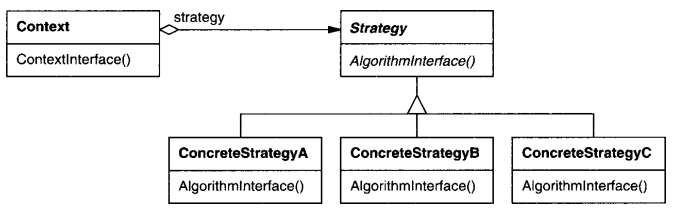
\includegraphics[scale=0.5]{5_padroes-contexto-funcional/5.3_comportamentais/5.3.09_strategy/diagram.png}
	\end{center}
\end{figure}

\subsection*{Exemplo Orientado a Objetos}

O exemplo do Strategy apresenta uma \textit{stream} 
de texto que pode ser quebrada em linhas utilizando 
estratégias diferentes. Nele, a classe Composition 
gerencia as quebras de linha do texto exibidas em 
um editor, enquanto a interface Compositor define 
uma estratégia de quebra de linha. As estratégias 
apresentadas são representadas pelas classes 
SimpleCompositor, TeXCompositor e ArrayCompositor. 
A implementação desse exemplo pode ser vista no código 
\ref{oostrategy}, enquanto o diagrama de classes pode 
ser visto na figura \ref{strategy_exemplo}.

\begin{figure}[htb]
	\caption{\label{strategy_exemplo}Exemplo de Strategy}
	\begin{center}
	    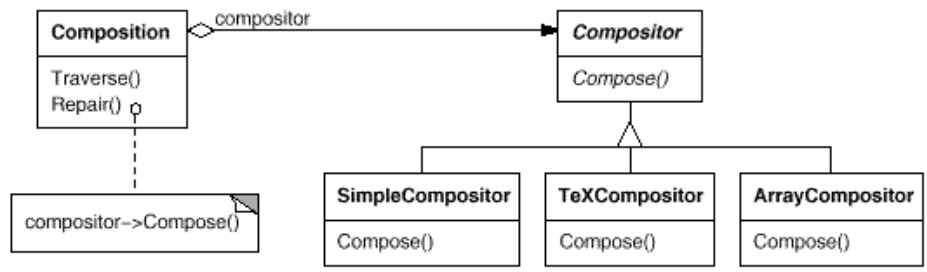
\includegraphics[scale=0.45]{5_padroes-contexto-funcional/5.3_comportamentais/5.3.09_strategy/exemplo_strategy.png}
	\end{center}
\end{figure}

\begin{lstlisting}[caption={Strategy Orientação a Objetos},label=oostrategy]
    
    trait Compositor {
        def compose(
            natural : Array(Coord), stretch : Array(Coord), shrink : Array(Coord),
            componentCount : Int, lineWidth : Int, breaks : Int
        ) : Int
    }

    class SimpleCompositor() extends Compositor {
        def compose(
            natural : Array(Coord), stretch : Array(Coord), shrink : Array(Coord),
            componentCount : Int, lineWidth : Int, breaks : Int
        ) : Int = {
            // implementação para SimpleCompositor
        }
    }

    class TeXCompositor() extends Compositor {
        def compose(
            natural : Array(Coord), stretch : Array(Coord), shrink : Array(Coord),
            componentCount : Int, lineWidth : Int, breaks : Int
        ) : Int = {
            // implementação para TeXCompositor
        }
    }

    class ArrayCompositor() extends Compositor {
        def compose(
            natural : Array(Coord), stretch : Array(Coord), shrink : Array(Coord),
            componentCount : Int, lineWidth : Int, breaks : Int
        ) : Int = {
            // implementação para ArrayCompositor
        }
    }

    class Composition(compositor : Compositor) {
        
        private var lineWidth : Int
        private var lineBreaks : Array[Int]
        private var lineCount : Int

        def repair() : Unit = {

            // Implementação da função repair

            val breakCount = compositor.compose(
                natural, stretchability, shrinkability,
                componentCount, _lineWidth, breaks
            )
    
        }

    }

\end{lstlisting}

\subsection*{Contexto Funcional}

No contexto funcional, a interface que define 
as operações que cada estratégia deve implementar 
não se faz necessária caso a função repair seja 
convertida em uma função de alta ordem que recebe 
como parâmetro uma função cuja assinatura seja 
igual à função compose. Dessa forma, qualquer 
função que possa implementar a quebra de linhas 
do exemplo pode ser passada por parâmetro sem 
que seja necessário implementar interfaces. 
A abordagem pode ser vista no código \ref{fpstrategy}.


\begin{lstlisting}[caption={Strategy Funcional},label=fpstrategy]
    
    def simpleCompose(
        natural : Array(Coord), stretch : Array(Coord), shrink : Array(Coord),
        componentCount : Int, lineWidth : Int, breaks : Int
    ) : Int = {
        // implementação para SimpleCompositor
    }

    def texCompose(
        natural : Array(Coord), stretch : Array(Coord), shrink : Array(Coord),
        componentCount : Int, lineWidth : Int, breaks : Int
    ) : Int = {
        // implementação para TeXCompositor
    }

    def arrayCompose(
        natural : Array(Coord), stretch : Array(Coord), shrink : Array(Coord),
        componentCount : Int, lineWidth : Int, breaks : Int
    ) : Int = {
        // implementação para ArrayCompositor
    }

    def repair(
        compose : (
            natural : Array(Coord), stretch : Array(Coord), shrink : Array(Coord),
            componentCount : Int, lineWidth : Int, breaks : Int) => Int
        ) : Unit {
        
        // Implementação da função repair
    
        val breakCount = compose(
            natural, stretchability, shrinkability,
            componentCount, _lineWidth, breaks
        )

    }
        

\end{lstlisting}


\subsection*{Vantagens e Desvantagens}

Utilizar funções de alta ordem no lugar do 
Strategy permite uma versatilidade maior quanto 
a que tipo de função pode ser aceita. Isso traz 
a vantagem de favorecer o reúso de funções que não 
foram planejadas para ser usadas como estratégias 
diferentes de implementação. Porém, traz a desvantagem 
de permitir que funções que possuam a mesma assinatura 
porém não realizem a operação desejada sejam passadas 
como estratégias válidas. Por exemplo, a função 
definida no código \ref{fpstrategyproblem} possui a 
mesma assinatura que as funções apresentadas no exemplo, 
mesmo que não esteja relacionada ao cálculo de quebras 
de linha.


 \begin{lstlisting}[caption={Strategy Funcional: Problema},label=fpstrategyproblem]
    
    def roundedModuleOfCrossProductVectors(
        vectors1 : Array(Coord), vectors2 : Array(Coord), vectors3 : Array(Coord),
        multiplier : Int, adder : Int, n_vecs : Int
    ) : Int = {
        // Retorna o módulo arredondado do produto vetorial 
        // entre os 3 grupos de N vetores recebidos, 
        // multiplicados por X e adicionado a Y
    }

\end{lstlisting}